\documentclass[../TST.tex]{subfiles}
\begin{document}
\begin{eproblem}[Bifilar torsional pendulum]{\ \\[5pt]}
\textit{Equipment:}\\
2 rulers (each of unknown mass $m$), 2 coins (each of mass $M=\qty{7.00}{g}$), tape measure, stopwatch, string, scissors, tape.\\

A bifilar torsional pendulum consists of a homogeneous rod of mass $m$ and length $L$ attached to two strings of length $h$ at points equidistant from the centre of mass. The distance between the strings is $d$. The pendulum oscillates with period $T$ about a vertical axis passing through its centre of mass. The moment of inertia $I$ of a rod of mass $m$ and length $l$ about an axis passing through its centre of mass perpendicularly to the rod is $I=\frac{1}{12}ml^2$. Record your results in the answer sheet.
\begin{figure}[h]
\centering
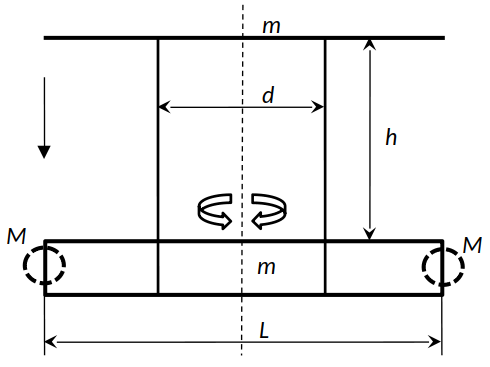
\includegraphics[width=0.6\textwidth]{fig/2016_e1.png}
\caption{}
\label{fig1}
\end{figure}

\begin{subpart}
	\item Find the centre of mass of the ruler. Write down the division of the ruler where it is located. What is the value of $L$ that you will be working with? \score{0.5} 
	\item Suspend the ruler as described above (see Figure \ref{fig1}, the plane of the ruler should be vertical). If the period $T$ depends on the length of the strings $h$ as $T\propto h^n$, find the number $n$ experimentally. Round your value to one of the numbers $\left(\pm\frac{1}{3},\pm\frac{1}{2},\pm 1,\pm 2,\pm 3\right)$. \phantom{aaaaahhhhh}\hfill\score{3.5}
	\item If the period $T$ depends on the distance between the strings $d$ as $T\propto d^k$, find the number $k$ experimentally. Round your value to one of the numbers $\left(\pm\frac{1}{3},\pm\frac{1}{2},\pm 1,\pm 2,\pm 3\right)$. \phantom{aaaaahhhhhh}\hfill \score{3.5}
	\item All in all, the period of the pendulum is given by
		\begin{equation*}
			T=2\pi C \frac{L}{\sqrt{g}} h^n d^k
		,
		\end{equation*}
	where $C$ is some number. Find the value of $C$ experimentally.	\score{3.5}
	\item Let the period of the pendulum be $T(0)$ for some constant $d$ and $h$.
		If we attach a coin to each end of the ruler (so that the centre of each coin is exactly on the rim of the ruler), the period becomes $T(M)$. The period of the pendulum $T(\mu)$ depends on its mass $\mu$ and its moment of inertia $I(\mu)$ as $T(\mu)\propto \sqrt{\frac{I(\mu)}{\mu}}$. Find a formula $m=f(M,T(0),T(M))$ from which the mass of the ruler $m$ can be determined. Take the necessary measurements and find $m$.\score{4.0}
\end{subpart}

\end{eproblem}
\end{document}
